\section{Related Work}
\frame{\sectionpage}


\begin{frame}[fragile]{SQL: Introduction}
    Given a SQL query, how is it executed?
    \begin{lstlisting}[language=SQL, caption= SQL query to execute.]
        SELECT MovieTitle
        FROM StarsIn
        WHERE StarName IN(
            SELECT name
            FROM MovieStar
            WHERE birthdate LIKE '%1960'
        );
    \end{lstlisting}
\end{frame}

\begin{frame}{SQL: Pipeline}
    \begin{figure}
        \centering
        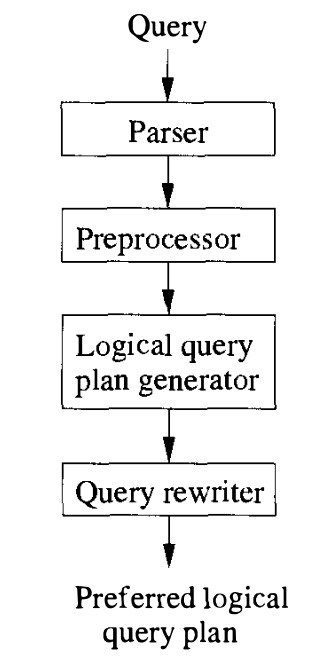
\includegraphics[scale=0.25]{query_processor.png}\\
        \caption{The pipeline for query processing}
        \label{fig:query_processor}
    \end{figure}
\end{frame}

\begin{frame}{SQL: Parser}
    \begin{figure}
        \centering
        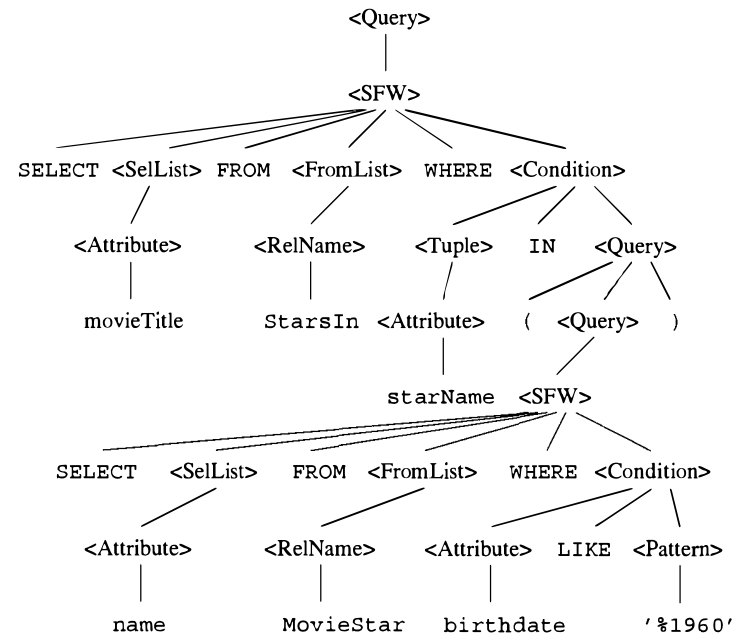
\includegraphics[scale=0.25]{parse_tree.png}\\
        \caption{An example of parse tree}
        \label{fig:prase_tree}
    \end{figure}
\end{frame}

\begin{frame}{SQL: Preprocessing}
    Sanity checking
    \begin{enumerate}
        \item Check relation uses
        \item Check and resolve attribute uses.
        \item Check types.
    \end{enumerate}
\end{frame}

\begin{frame}{SQL: Relational Algebra}
    \begin{figure}
        \centering
        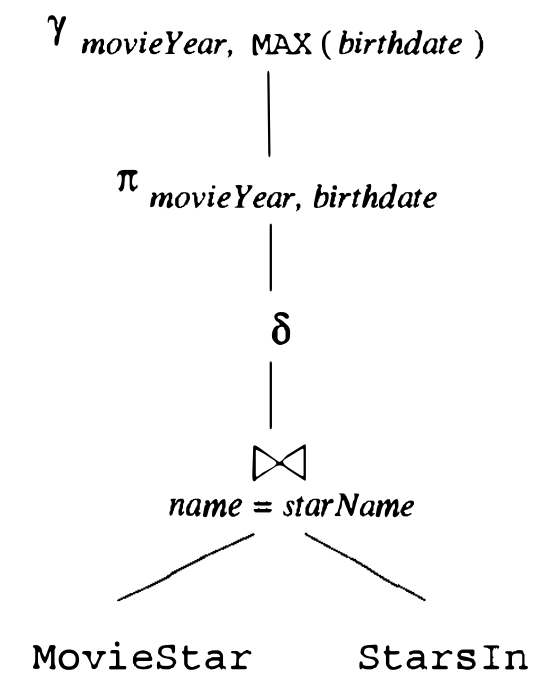
\includegraphics[scale=0.25]{join_pushdown1.png}\\
        \caption{An example of join being optimized}
        \label{fig:j_1}
    \end{figure}
\end{frame}

\begin{frame}{SQL: Relational Algebra}
    \begin{figure}
        \centering
        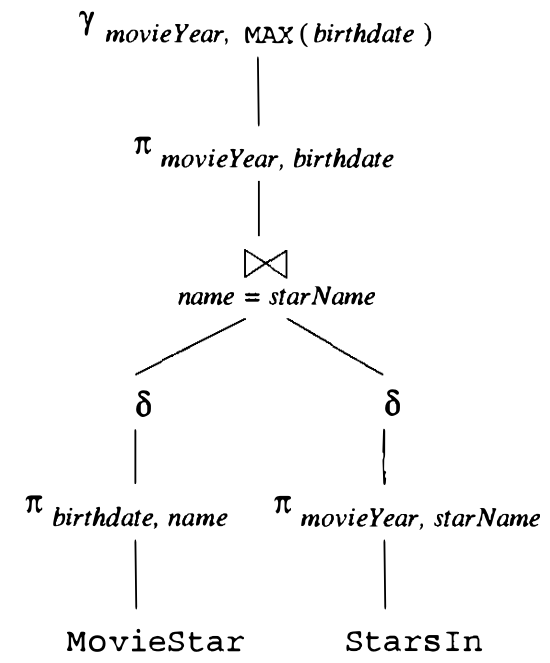
\includegraphics[scale=0.25]{join_pushdown2.png}\\
        \caption{An example of Relational Algebra being used for optimization}
        \label{fig:j_2}
    \end{figure}
\end{frame}

\begin{frame}{SQL: Rewrite}
    Need to convert the query plan using Relational Algebra into a query plan which requires has lowest cost according to estimates.
\end{frame}

\begin{frame}{SQL: Cost: Estimation}
    \begin{enumerate}
        \item Give accurate estimates. No matter what method is used for executing query plans.
        \item Are easy to compute.
        \item Are logically consistent.
    \end{enumerate}
\end{frame}

\begin{frame}{SQL: Cost: Methods}
    \begin{enumerate}
        \item Histogram
        \item Heuristics
        \item Top-Down
        \item Bottom-up
        \item Dynamic Programming
        \item Branch-and-Bound
        \item Hill Climbing
        \item Selinger-Style Optimization
    \end{enumerate}
\end{frame}

\begin{frame}{SQL: Cost: Considerations}
    \begin{enumerate}
        \item An order and grouping for associative-and-commutative operations
        \item An algorithm for each operator
        \item Additional operators - scanning, sorting
        \item The way in which arguments are passed    
    \end{enumerate}
\end{frame}

\begin{frame}{SQL: Joins}
    \begin{enumerate}
        \item Algorithm Nested-loop join
        \item Algorithm Index join
        \item Order Dynamic Programming
        \item Order Greedy
    \end{enumerate}
\end{frame}

\begin{frame}{SQL: Physical Plan}
    \begin{enumerate}
        \item Selection, Index based
        \item Selection, Table Scan
        \item Join, One-pass join
        \item Join, Hash join
        \item Join, Index join
    \end{enumerate}
\end{frame}

\begin{frame}{Stream Query Optimization}
    Modifying queries by changing graph topology and/ or operators to get better performance, as measured by
    \begin{enumerate}
        \item Throughput
        \item Latency
        \item Resource Usage.
    \end{enumerate}
    While preserving semantice of the original query.
\end{frame}

\begin{frame}{Stream Graph}
    Queries on Data streams can be thought of as directed graphs,
    \begin{enumerate}
    \item Edges represent streams and nodes represent operators.
    \item Root  and  leaf nodes are called sources and sinks, respectively.
    \end{enumerate}
    Whereas for traditional Databases, we have parse trees.
\end{frame}

\begin{frame}{Possible Optimizations}
    \begin{itemize}
        \item Batching
        \item Placement
        \item State sharing
        \item Load Balancing
        \item Algorithm selection
        \item Load Shedding
        \item Fusion
        \item Operator Separation
        \item Operator Reordering
        \item Redundancy elimination
        \item Fission
    \end{itemize}
\end{frame}

\begin{frame}{Operator Reordering}
    A reordering operator moves more selective operators, which reduce the data volume upstream. This has the benefit of reducing the amount of data flowing into downstream compuration. Thus eliminatin unnecessary work. 
    We focus on finding the optimal method of executing associative opeators.
\end{frame}

\begin{frame}{Research Question}
    \begin{center}
    Is it possible to apply deep reinforcement learning to find the optimal ordering of executing associative operations?
    \end{center}
\end{frame}

\begin{frame}{Deep Neural Networks}
    Deep neural networks is a layer wise combinations of neurons\\
    Building up on the neuron seen in the last slide. We have
    \begin{figure}
        \centering
        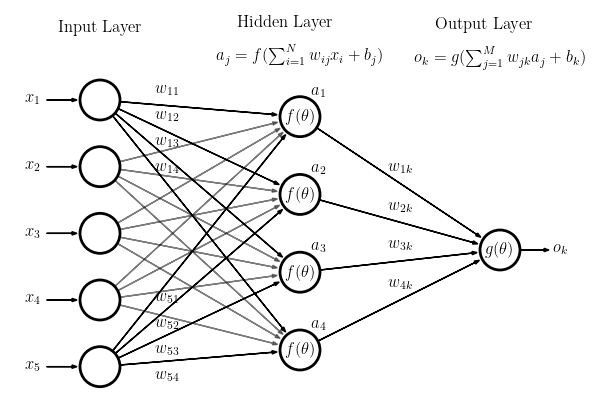
\includegraphics[scale=0.5]{dl.png}\\
        \caption{Example of a deep neural network}
        \label{fig:dl}
    \end{figure}
\end{frame}

\begin{frame}{Reinforcement Learning}
    What is reinforcement learning? How is it different from supervised and unsupervised learning?
    \begin{figure}
        \centering
        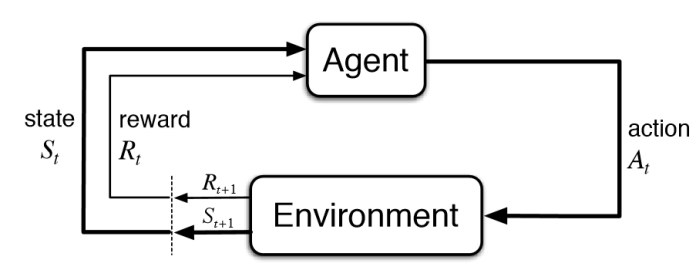
\includegraphics[scale=0.5]{rl.jpg}\\
        \caption{Example of a framework of a reinforcement learning agent }
        \label{fig:rl}
    \end{figure}
\end{frame}

\begin{frame}[fragile]{Optimal Policy}
    \begin{lstlisting}[language=python, caption=value iteration algorithm]
    for s in S:
        V(s)=0
    while(not converged):
        for s in S:
            V(s)=R(s)+max over all action[gamma*(sum(P(s,a,s')V(s')))]
    \end{lstlisting}
    
    \begin{lstlisting}[language=python, caption=Policy iteration algorithm]
    initialize random pi
    while(not converged):
        V=V(pi)
        for s in S:
            pi(s)=max over all actions[sum(P(s,a,s')V(S'))]
    \end{lstlisting}
\end{frame}

\begin{frame}{Deep Reinforcement Learning}
    Deep reinforcement learning combines Deep learning and reinforcement learning
    \begin{figure}
        \centering
        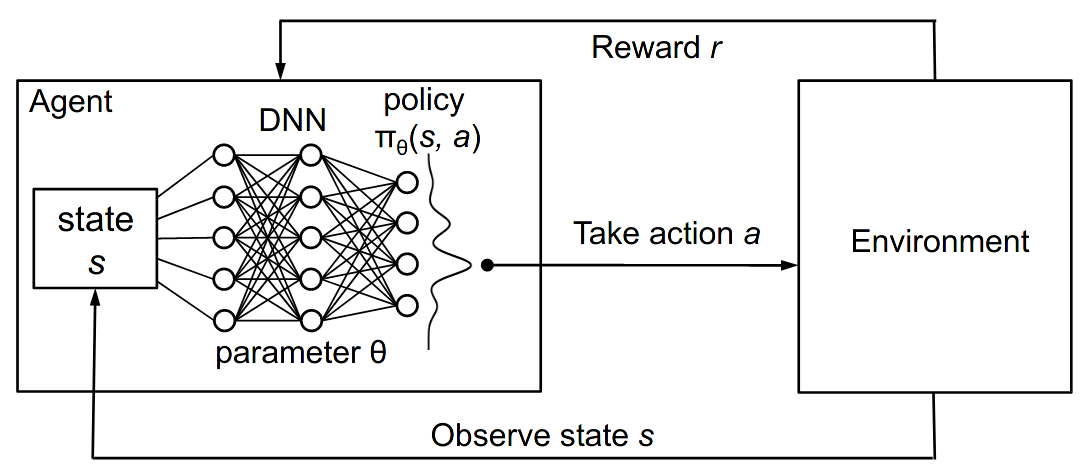
\includegraphics[scale=0.25]{drl.png}\\
        \caption{Deep Reinforcement learning(DQN) framework}
        \label{fig:drl}
    \end{figure}
\end{frame}
